\documentclass[a4paper,12pt]{article}
\usepackage{enumitem} % -> Alphabetical Lists
\usepackage{amsmath} % -> Matrices
\usepackage{fullpage} % -> A4 Full Page
\usepackage{amssymb} % -> Therefore
\usepackage[utf8]{inputenc}
\usepackage{graphicx}
\usepackage{adjustbox}
\usepackage{listings}
\usepackage{braket}
\usepackage{geometry}
\usepackage{tikz}
\usepackage{gensymb}
\usepackage{dirtytalk}
\graphicspath{ {./images} }


\usetikzlibrary{quantikz}

\graphicspath{ {./} }

\geometry{
    a4paper,
    total={175mm,257mm},
    left=20mm,
    top=20mm,
}

\title{Quantum Computing Assignment 9 - Group 18}
\author{
    Rallabhandi, Anand Krishna 
    \and
    Mustafa, Syed Husain
    \and
     , Mohammed Kamran 
}
\date{\today}

\begin{document}

\maketitle

\section*{Exercise 9.1}

 \begin{large}(\textbf{Phase Estimation})
 \end{large}

\begin{enumerate}[label=(\alph*)]
\item The Quantum Fourier Transform acts on a quantum state $\sum\limits_{k=0}^{N-1}x_{i}\ket{i}$ and maps it to the quantum state $\sum\limits_{k=0}^{N-1}y_{i}\ket{i}$ according to the formula:
\[y_{k} = \frac{1}{\sqrt{N}}\sum\limits_{j=0}^{N-1}x_{j}e^{2\pi ijk/N} \hspace{10mm} \textbf{(A)}\]
Similarly the formula for Inverse Quantum Fourier Transform is given by: 
\[x_{j} = \frac{1}{\sqrt{N}}\sum\limits_{k=0}^{N-1}y_{k}e^{-2\pi ijk/N} \hspace{10mm} \textbf{(B)}\]
Applying \textbf{(A)} to a single qubit state $\ket{\psi} = \alpha\ket{0}+\beta\ket{1}$: \\
$y_0 = \frac{1}{\sqrt{2}}\Big(\alpha e^{2\pi i \frac{0\times 0}{2}}+ \beta e^{2\pi i \frac{1\times 0}{2}}\Big) = \frac{1}{\sqrt{2}}(\alpha+\beta)$ \& $y_1 = \frac{1}{\sqrt{2}}\Big(\alpha e^{2\pi i \frac{0\times 1}{2}}+ \beta e^{2\pi i \frac{1\times 1}{2}}\Big) = \frac{1}{\sqrt{2}}(\alpha-\beta)$\\
$U_{QFT}\ket{\psi}  = \frac{1}{\sqrt{2}}(\alpha+\beta)\ket{0} + \frac{1}{\sqrt{2}}(\alpha-\beta)\ket{1}= \ket{\tilde{\psi}} \hspace{10mm} \textbf{(C)} $\\~\\
The above result is the same as applying the Hadamard Operator \textbf{(H)} on the qubit.\\
$\therefore$ \underline{Circuit for Forward Fourier Transform}: \begin{quantikz}
    \lstick{$\ket{\psi}$} & \gate{H}&\qw \rstick{$\ket{\tilde{\psi}}$}\\
\end{quantikz}  \\
Applying \textbf{(B)} on \textbf{(C)} :\\
$x_0 = \frac{1}{\sqrt{2}}\Big(\frac{\alpha+\beta}{\sqrt{2}} e^{-2\pi i \frac{0\times 0}{2}}+ \frac{\alpha-\beta}{\sqrt{2}} e^{-2\pi i \frac{0\times 1}{2}}\Big) = \alpha$ \& $x_1 = \frac{1}{\sqrt{2}}\Big(\frac{\alpha+\beta}{\sqrt{2}} e^{-2\pi i \frac{1\times 0}{2}}+ \frac{\alpha-\beta}{\sqrt{2}} e^{-2\pi i \frac{1\times 1}{2}}\Big) = \beta$ \\
$U_{IQFT}\ket{\psi}$ = $\alpha\ket{0}+\beta{\ket{1}}$  \textbf{(D)}\\
The above result is the same as applying Hadamard Gate to the \textbf{(C)}.\\
$\therefore$ \underline{Circuit for Inverse Fourier Transform}:  \begin{quantikz}
    \lstick{$\ket{\tilde{\psi}}$} & \gate{H}&\qw \rstick{$\ket{\psi}$}\\
\end{quantikz}  \\ \pagebreak

\item
\[\begin{quantikz}
    \lstick{$\ket{0}$} & \gate{H} & \ctrl{1} & \gate{\text{$\mathcal{F} ^{-1}$}} & \meter{} &\qw\\
    \lstick{$\ket{\psi}$}& \qw\qwbundle[alternate]{} & \gate{U}\qwbundle[alternate]{} & \qwbundle[alternate]{} & \qw\qwbundle[alternate]{} & \qw\qwbundle[alternate]{}\\
\end{quantikz}\]
Let $\ket{-1}$ \& $\ket{1}$ be the eigen states of U with eigen values $\pm1$. We apply the above circuit operations and obtain the following states: \\
$\ket{\psi_{0}} = \sum\limits_{j=-1,1}c_{i}\ket{0}\ket{j}$ : Before Applying Any Operation.\\
$\ket{\psi_{1}} = \sum\limits_{j=-1,1}c_{i}\frac{1}{\sqrt{2}}\sum\limits_{k=0,1}\ket{k}\ket{j}$ : After Applying the Hadamard Gate. \\
$\ket{\psi_2} = \sum\limits_{j=-1,1} c_{i}\frac{1}{\sqrt{2}}\Big(\ket{0} + e^{2\pi i \varphi_i} \ket{1}\Big)\ket{j}$ : After Applying Controlled-U Operator.\\
$\ket{\psi_3} = \sum\limits_{j=-1,1} c_{i}\ket{\varphi_i}\ket{j}$ : After Applying Inverse Fourier Transform to obtain Phase $\varphi$\\~\\
When performing the measuring operation on $\ket{\psi_3}$ the second qubit collapses into one of the eigenstates of U. When the first qubit is measured to be $\ket{0}$ the final state of second qubit is $\ket{+1}$, and when the first qubit is $\ket{1}$ it is $\ket{-1}$. This implies that Phase Estimation applied to a one bit register is equivalent to \say{Measuring an Operator} as shown in Tutorial 3.


\end{enumerate} 
\section*{Exercise 9.2}

 \begin{large}(\textbf{Order Finding}) \\~\\
 \end{large}
    \begin{enumerate}[label=(\alph*)]

    \item 
    \begin{gather*}
        \frac{1}{\sqrt{r}} \sum_{s=0}^{r-1} e^{2\pi isk/r}|u_s\rangle = \\~\\
        \frac{1}{r}\sum_{s=0}^{r-1} \sum_{k_2=0}^{r-1} e^{2\pi is(k-k_2)/r} |x^{k_2}(mod N)\rangle\\~\\
        = \sum_{k_2=0}^{r-1} \delta |x^{k_2}(mod N)\rangle\\~\\
        = |x^{k}(mod N)\rangle
    \end{gather*}
\item \begin{gather*}
    7^1 \equiv 7 \hspace{0.1cm} mod \hspace{0.1cm} 15 \\~\\
    7^2 \equiv 4 \hspace{0.1cm} mod \hspace{0.1cm} 15 \\~\\
    7^3 \equiv 13 \hspace{0.1cm} mod \hspace{0.1cm} 15 \\~\\
    7^4 \equiv 1 \hspace{0.1cm} mod \hspace{0.1cm} 15 \\~\\
    \end{gather*}
    Therefore $r = 4$
    \begin{gather*}
    |\chi\rangle = \frac{1}{\sqrt{2^t}}\sum_{j=0}^{2^t - 1 }|j\rangle |x^j mod N\rangle\\~\\
    \end{gather*} \\
    For $t=5$, we get

    \begin{gather*}
    |\chi\rangle = \frac{1}{\sqrt{2^5}}[|0\rangle |7^0 mod 15\rangle + |1\rangle |7^1 mod 15\rangle + |2\rangle |7^2 mod 15\rangle + |3\rangle |7^3 mod 15\rangle + ......\\....+|31\rangle |7^{31} mod 15\rangle ]  \\~\\
    |\chi\rangle = \frac{1}{\sqrt{2^5}}[|0\rangle |7^0 mod 15\rangle + |1\rangle |7^1 mod 15\rangle + |10\rangle |7^2 mod 15\rangle + |11\rangle |7^2 mod 15\rangle + ......\\....+|11111\rangle |7^{31} mod 15\rangle ]
    \end{gather*}

\item When we select $\ket{4}$ as the basis state for the second qubit, then we can only select values that produce 4 mod 15.\\
We know $7^2$ = 4 mod 15, as the period of function $f: k \rightarrow 7^k$ mod 31 is 4, then $\forall k \geq 1$ we select $7^{2+4k}$ mod 15.\\
From \textbf{(b)} we have 8 such powers of 7, ie; $7^2, 7^6, 7^{10}, 7^{14}, 7^{18}, 7^{22}, 7^{26}, \&$ $7^{30}.$\\
$\ket{\chi'} = \frac{1}{\sqrt{2^5}}\sum\limits_{j=0}^{7}\ket{2+4j}\ket{4}$ \\
$\|\chi'\| = \sqrt{\frac{1}{32}+\frac{1}{32}+\frac{1}{32}+\text{8 times ...}} = \sqrt{\frac{8}{32}}=\frac{1}{2}$\\~\\
\underline{Normalized $\ket{\chi'}$} : $\frac{\ket{\chi'}}{\|\chi'\|}$ = $\frac{2}{\sqrt{2^5}}\sum\limits_{j=0}^{7}\ket{2+4j}\ket{4}= \frac{1}{\sqrt{2^3}}\sum\limits_{j=0}^{7}\ket{2+4j}\ket{4}$\pagebreak
\item     \phantom{-}\\\graphicspath{./images}
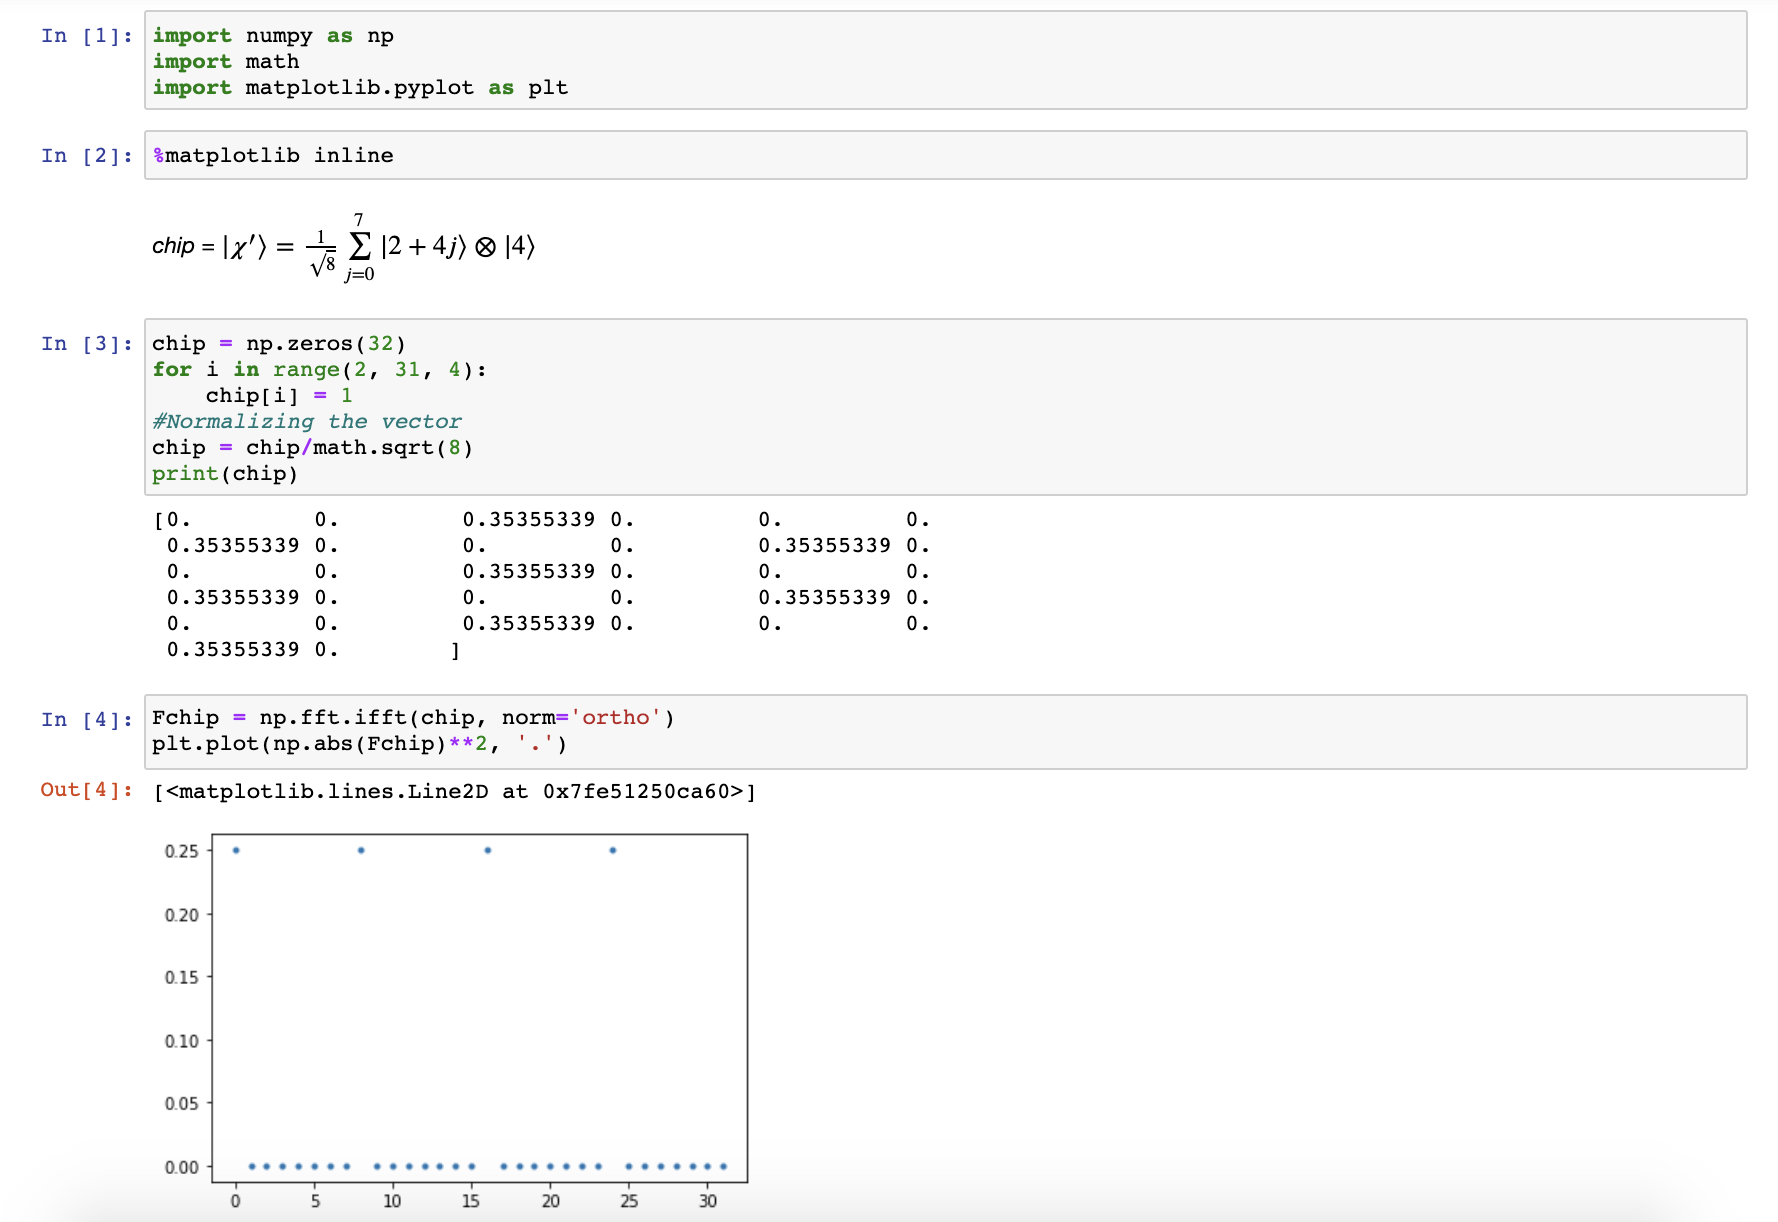
\includegraphics[scale=0.50]{images/img.png}\\~\\
\end{enumerate}
\end{document}
